% !TeX program = lualatex
\documentclass[french,twocolumn,twoside]{article}
\usepackage{fontspec}
\usepackage[compact]{titlesec}
\usepackage{amsmath}
\usepackage{enumitem}
\usepackage{aurical}
\usepackage[top=1.75cm,bottom=1.8cm,left=2cm,right=2cm,a4paper,includehead,includefoot,heightrounded]{geometry}
\usepackage{babel}
\usepackage{xcolor}%
\usepackage[colorlinks=true,
			linkcolor=blue!50!red,
			urlcolor=brown!60!black,
			pdfauthor={Altay},
			pdftitle={Clés et pièces},
			pdfsubject={Un mini jeu de rôles à thème Fort Boyard},
			pdfcreator={LaTeX}]{hyperref}
\usepackage{graphicx}
\usepackage{xspace}
\usepackage{pifont}
\usepackage{fontawesome}
\usepackage{fancyhdr}
\usepackage{lettrine}
\usepackage{Typocaps}
\usepackage{background}
\usepackage{microtype}
\usepackage{siunitx}
\usepackage{pgfornament}
\usepackage{multicol}

\newcommand\fboyard{{\fontspec{Serpentine Medium} \textsc{Clés et pièces}}\xspace}
\newcommand\animateur{{\fontspec{Serpentine Medium} \textsc{Animation}}\xspace}
\newcommand\equipe{{\fontspec{Serpentine Medium} \textsc{Équipe}}\xspace}
\newcommand\cervo{{\Fontlukas\large\textsc{Cervo}}\xspace}
\newcommand\kosto{{\Fontlukas\large\textsc{Kosto}}\xspace}
\newcommand\gueulo{{\Fontlukas\large\textsc{Beuglo}}\xspace}
\newcommand\key{{\faKey}\xspace}
\newcommand\info{{\faInfo}\xspace}
\newcommand\bulb{{\faLightbulbO}\xspace}
\newcommand\fist{{\faHandRockO}\xspace}
\newcommand\cristal{{\faDiamond}\xspace}

\input Kramer.fd
\newcommand*\initfamily{\usefont{U}{Kramer}{xl}{n}}

\pagestyle{fancy}
\fancyhf{}
\fancyhead[L]{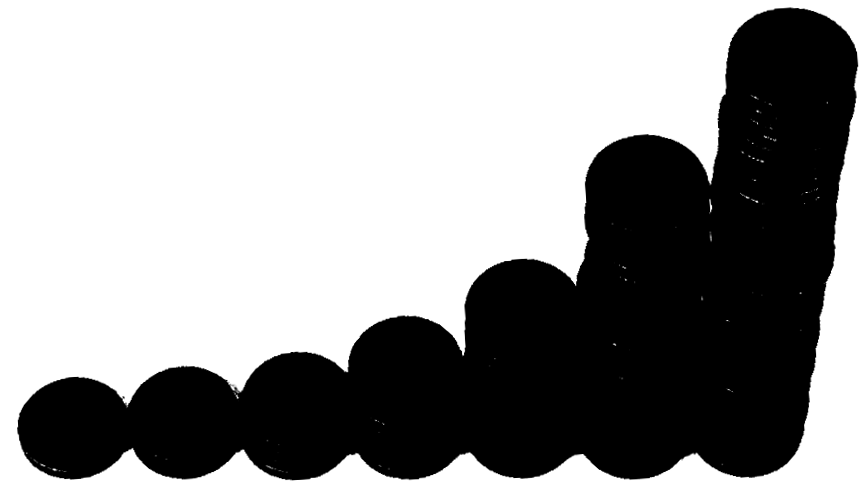
\includegraphics[height=1em]{piece} \fboyard}
\fancyhead[R]{Un mini jeu de rôles par Altay}
\fancyhead[C]{\pgfornament[width=4cm]{86}}
\fancyfoot[C]{\pgfornament[width=2cm]{158}}
\fancyfoot[RO,LE]{\thepage}

\renewcommand{\headrulewidth}{0pt}
\renewcommand{\footrulewidth}{0pt}

\backgroundsetup{
	scale=1,
	color=black,
	opacity=0.15,
	angle=0,
	contents={%
		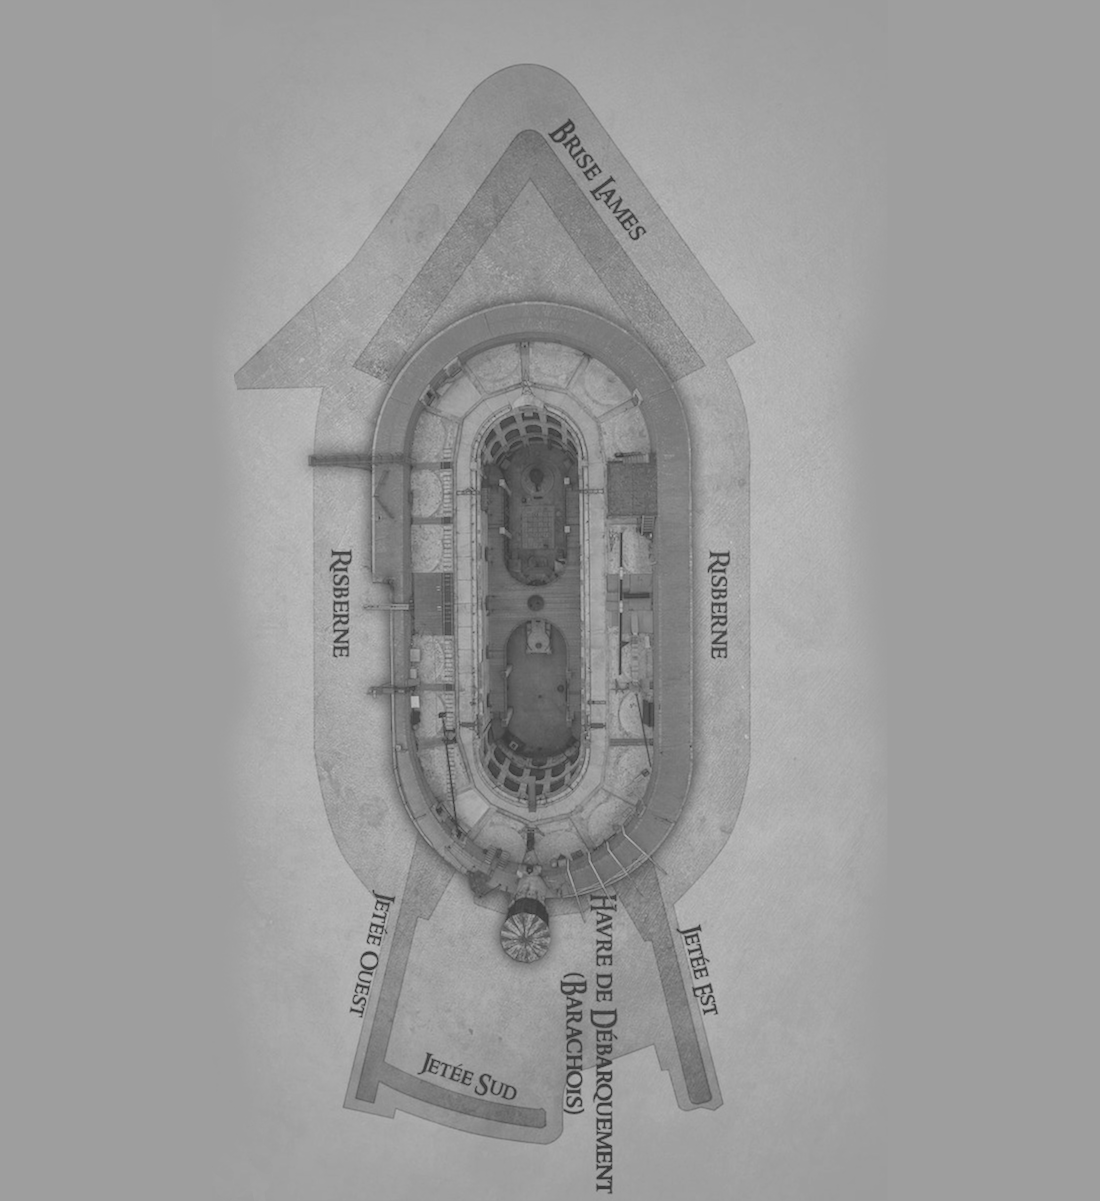
\includegraphics[height=\paperheight]{background}
	}%
}

\newcommand{\eachpageornament}{%

\begin{tikzpicture}[remember picture, overlay]
\node[anchor=north west] at (current page.north west){%
\pgfornament[width=2cm]{37}};%
\node[anchor=north east] at (current page.north east){%
\pgfornament[width=2cm,symmetry=v]{37}};%
\node[anchor=south west] at (current page.south west){%
\pgfornament[width=2cm,symmetry=h]{37}};%
\node[anchor=south east] at (current page.south east){%
\pgfornament[width=2cm,symmetry=c]{37}};%
\end{tikzpicture}
}

\setsansfont[Ligatures=TeX]{Copperplate Gothic Bold}
%\setsansfont[Ligatures=TeX]{Serpentine Medium}


\titleformat{\section}
	{\normalfont\sffamily\Large\bfseries}
	{\thesection}{1em}{}

\titleformat{\subsection}
	{\normalfont\sffamily\large\bfseries}
	{\thesubsection}{1em}{}

\renewcommand{\LettrineFontHook}{\initfamily}
	
\begin{document}
\eachpageornament%

\includegraphics[width=0.4\textwidth]{logo}

\setlength\parindent{0pt}

\fboyard est un jeu de rôles sur table estival, conçu pour occuper entre une et deux heures au moment de l'apéro à l'aide d'un dé à dix faces (d10) et quelques bouts de papier.

\section*{Le casting}

\subsection*{Équipe et animation}

\lettrine{D}{ans} \fboyard, les joueuses incarnent des personnalités mineures du PAF, des artistes, journalistes ou sportives en perte de vitesse de la fin des années 90 ou des stars montantes du début des années 2000. La fine équipe se réunit pour vider la salle au trésor d'un fort insulaire dans un jeu télévisé caritatif animé par Olivier Minne et Sarah Lelouch.

La tablée désigne de façon collégiale une personne pour prendre le rôle de l'\animateur. Si aucune joueuse ne fait l'unanimité, on choisit la plus musclée.

Les joueuses restantes forment l'\equipe et choisissent un nom ainsi qu'une association dont elles souhaitent faire avancer la cause, par exemple la fondation ``Un enfant, un manteau'' (\textit{amenez un enfant, repartez avec un manteau}).

Chaque personnalité est caractérisée par trois attributs, notées par une valeur de 1 à 9:
\begin{itemize}
	\item[\ding{71}] \cervo: sert pour les énigmes et les jeux,
	\item[\ding{71}] \kosto: sert pour les épreuves physiques,
	\item[\ding{71}] \gueulo: sert pour encourager les autres.
\end{itemize}

Les joueuses distribuent 15 points dans les attributs. Lors des épreuves, on lance le d10: si le résultat du dé est inférieur ou égal à l'attribut, c'est un succès, sinon, c'est un échec. On peut forcer l'utilisation d'un autre attribut pour une épreuve en le diminuant définitivement de 1.

\subsection*{Habitants du fort}

\lettrine{Q}{uelques} personnages non-joueurs viennent prêter main-forte à l'\animateur:
\begin{itemize}
	\item[\faQuestion] Le Père Fouras pose des énigmes à aux candidats et candidates qui visitent sa vigie.
	\item[\faLock] La Boule enferme les personnalités malchanceuses aux épreuves dans ses geôles.
	\item[{\faMale\faMale}] Passe-Partout et Passe-Temps guident l'équipe de salle en salle à travers le fort.
	\item[\faPaw] Felindra la dresseuse de tigres garde l'accès à la fontaine à boyards.
	\item[\fontspec{DejaVu Sans} 😾] Les Maîtres du Temps forment le Conseil, anonymes sous leur masque de tigre.
\end{itemize}


\section*{L'émission}

\lettrine{O}{n} utilise les règles de l'émission Fort Boyard saisons 2003 à 2006 (présentée par Olivier Minne et Sarah Lelouch)\footnote{Les règles sont sensiblement les mêmes que la version 2007 à 2009 (présentée par Olivier Minne, mais avec Anne-Gaëlle Riccio) ou que celles des saisons 2000 à 2002 (présentées par Jean-Pierre Castaldi et Cendrine Dominguez). Vous pouvez adapter le déroulement de l'émission à n'importe quelle autre saison, mais débrouillez-vous, je peux pas tout faire.}. De manière générale, on ne joue pas tant les épreuves que ce qui se passe à l'extérieur et les échanges quand l'\equipe galope dans le fort.
Les membres de l'équipe se motivent et poussent leur cri de guerre, l'\animateur souhaite la bienvenue aux téléspectateurs, on lance le \href{https://youtu.be/7dtDD3D4A7E}{générique}.

L'émission est découpée en quatre séquences:
\begin{enumerate}
	\item[\ding{172}] Les épreuves,
	\item[\ding{173}] La salle du Conseil,
	\item[\ding{174}] Les aventures,
	\item[\ding{175}] La salle du trésor.
\end{enumerate}

\subsection*{Les épreuves}

\lettrine{D}{urant} les épreuves, l'\equipe tente d'amasser des clés \key qui serviront à accéder à la salle du trésor.

À tour de rôle, l'\animateur désigne une personnalité qui accomplit l'épreuve, inventée ou choisie dans la liste en annexe.

La joueuse désignée effectue un jet de dé sur l'attribut associé à l'épreuve.

\begin{itemize}
	\item[\faThumbsOUp] Succès: l'épreuve rapporte 1 \key, la joueuse décrit sa réussite,
	\item[\faThumbsODown] Échec: la personnalité est enfermée aux oubliettes par la Boule, la joueuse décrit son échec.
\end{itemize}

Une autre joueuse peut sacrifier de façon définitive un point de \gueulo pour:
\begin{itemize}
	\item[\faCommentO] Avant une épreuve: faire le jet à la place d'une autre joueuse (``\textit{Ralentis, étends les bras, pousse avec les jambes!}'').
	\item[\faHourglassEnd] Après une épreuve: faire sortir le personnage d'une autre joueuse avant la fin de la clepsydre et lui éviter les oubliettes (``\textit{Sors, sors! T'as plus le temps!}'').
\end{itemize}

Entre deux épreuves, l'\equipe court derrière Passe-Partout pour rejoindre la salle suivante. C'est l'occasion d'échanger quelques mots, de se faire beau pour la caméra ou de pousser un cri de guerre.

Les personnages aux oubliettes y restent jusqu'à leur libération mais continuent à être filmés (``\textit{Coucou maman!}'').

Les épreuves se terminent soit au bout de 45 minutes de jeu IRL, soit après 15 épreuves, soit quand l'\equipe a obtenu 7 clés {\faKey}.

\subsection*{La salle du Conseil}
\eachpageornament%

\lettrine{L}{e} cristal \cristal permet d'accéder à la salle du Conseil. Sa récupération est le fait d'une longue épreuve de groupe, souvent en relais. L'\animateur désigne secrètement une personnalité et note son nom sur un bout de papier. Toutes les joueuses de l'\equipe lancent le dé. Si le personnage désigné par l'\animateur obtient le plus petit score, l'\equipe échoue son défi et perd le cristal. On passe alors immédiatement aux aventures.

Si l'\equipe met la main sur le cristal, elle peut ouvrir la porte de la salle du Conseil où celui-ci les attend de pied ferme. Il est de bon ton pour l'\animateur de garder les bras croisés de façon stoïque et autoritaire tout au long de cette phase.

L'\equipe choisit quelle personnalité (hors oubliettes) participera au duel \textbf{avant} que l'\animateur ne dévoile l'épreuve choisie par le Maître du Temps qu'elle devra affronter. Chaque victoire contre un Maître rapporte soit la libération d'un prisonnier, s'il y en a encore, soit 30 secondes de temps additionnel pour la salle du trésor. L'\equipe ne peut pas utiliser de point de \gueulo pendant cette phase. Les prisonniers non libérés dans la salle du Conseil sont coincés jusqu'à la fin du jeu. Dommage pour leur temps de présence à l'écran!

On effectue 4 duels avant de passer à la suite.

\subsection*{Les aventures}

\lettrine{L}{es} aventures sont des épreuves permettant d'obtenir des indices {\faInfo} concernant le mot-code nécessaire pour ouvrir la fontaine à boyards. L'\animateur invente ou choisit une aventure dans la liste. Si la joueuse désignée réussit, elle récupère un indice {\faInfo} plutôt qu'une clé. Les aventures sont bien plus spectaculaires que les épreuves: attraper un bout de papier sur une mygale, faire du saut à l'élastique, bref, c'est le moment d'en faire des caisses pour être sûr de passer au zapping.

La phase d'aventures s'arrête au bout de 6 épreuves ou de 20 minutes de temps de jeu IRL.

\subsection*{La salle du Trésor}

\lettrine{P}{our} entrer dans la salle du trésor et amasser le pactole, il faut au minimum 5 clés {\faKey} et le mot-code.

Déterminer le mot-code demande 6 points de réflexion {\faPuzzlePiece}, à raison de $1~\text{\faInfo} = 1~\text{\faPuzzlePiece}$.

L'\equipe a 4 minutes plus tout le temps additionnel accumulé dans la salle du Conseil. Elle peut choisir d'emprisonner une des personnalités pour obtenir un {\faInfo} ou une {\faKey} supplémentaire.

À partir de 3 indices, l'\equipe peut sacrifier une minute de temps contre 1 {\faPuzzlePiece} additionnel.

\href{https://youtu.be/tHu4Kd_eel0}{La porte de la salle du trésor s'ouvre} quand l'équipe a obtenu 6 {\faPuzzlePiece}.

Pour chaque tranche de 30 secondes restantes, les joueuses libres ramassent des boyards:
\begin{itemize}
	\item[\ding{223}] Avec 5 {\faKey}, la porte n'est ouverte que de \SI{50}{\centi\meter}: chaque joueuse lance 2d10 et conserve le pire résultat,
	\item[\ding{224}] Avec 6 {\faKey}, la porte n'est ouverte que de \SI{120}{\centi\meter}: chaque joueuse lance 1d10,
	\item[\ding{225}] Avec 7 {\faKey}, la porte est complètement ouverte: chaque joueuse lance 2d10 et conserve le meilleur résultat.
\end{itemize}

Chaque point de \gueulo non dépensé à ce stade ajoute 1d10 boyards à la cagnotte.

On calcule ensuite le montant reversé à l'association: nombre de boyards $\times$ 100 euros.

Si on n'a pas pu braquer le trésor, alors on se réconforte en se disant que l'essentiel c'était de faire connaître l'association.

Sinon, on saute de joie quand le montant s'affiche.

\href{https://www.youtube.com/watch?v=BnYDldFEqk4}{\textit{Générique de fin.}}

\section*{(optionnel) La promo}

\lettrine{S}{i} vous voulez épiloguer, chaque personnalité est invitée à résumer son expérience du fort dans une émission de divertissement\footnote{Pensez Michel Drucker/Denisot, Thierry Ardisson ou Sophie Favier. Cyril Hanouna est formellement \textbf{interdit}, n'y pensez même pas.} et raconter à quel point c'était formidable d'aider les autres.

L'\animateur conclut par un commentaire sur la performance de l'équipe (``\textit{En fait, pour rendre les gens heureux sur le fort, il faut les faire courir, leur faire peur, les maltraiter! À bientôt pour une nouvelle émission, toujours plus loin, toujours plus haut, toujours plus\dots FORT!}'').

\section*{Règles alternatives}

\subsection*{Vraie énigme}

L'\animateur peut préparer une véritable énigme dans son coin avec jusqu'à six indices. Généralement, il s'agit de faire trouver un mot dénominateur commun d'une liste (par exemple, ``tube'' pour ``essai, cylindre, chanson, succès, peinture, pneumatique'').

Plutôt que de dépenser du temps de réflexion pour trouver le mot-code, jouez la dernière phase en temps réel.

\subsection*{Pas de quartier}

Certaines épreuves génèrent des prisonniers si on les échoue car il est impossible de sortir. Par exemple, l'épreuve de la menotte implique de se faire attacher à un tuyau: impossible de sortir avant l'épuisement de la clepsydre. L'\animateur peut inclure quelques épreuves de ce type pour corser la difficulté.

\subsection*{Épreuves à plusieurs}

Quelques épreuves de Fort Boyard se font à deux. Dans ce cas là, deux joueuses lancent le dé\dots{} Deux fois plus de compagnie pour la Boule!

\subsection*{Trop/pas assez de joueuses}

À la louche, le jeu devrait être adapté pour une tablée de 5 à 9 personnes. Il faut viser entre 4 et 8 membres dans l'\equipe.

Trop de joueuses? Distribuez-leur les multiples rôles endossés par l'\animateur: l'animatrice qui coache l'équipe (là où l'animateur est plutôt un adversaire\footnote{Cf. note d'intention.}) et les habitants du fort, en commençant par Passe-Partout/Passe-Temps qui collent aux basques des candidats et candidates. Ils sont muets dans l'émission, mais hé, sachez improviser.

Pas assez de joueuses? Donnez deux personnalités par membre de l'\equipe, ça devrait bien se passer.

\eachpageornament%
\section*{Annexes}

\subsection*{Liste des épreuves \key} \url{https://www.fort-boyard.fr/epreuves.php#sortBy=chrono&filter=.eprE.s2004}

On liste ici les 35 épreuves de la saison 2004 en guise d'exemple.
\fist = \kosto, \bulb = \cervo
\begin{minipage}{0.5\textwidth}
\begin{multicols}{2}
\begin{enumerate}
	\item Bonneteau \bulb
	\item Étriers suspendus \fist
	\item Jarres aux souris \bulb
	\item Lutte dans la boue \fist
	\item Mur glissant \fist
	\item Père Fouras \bulb
	\item Tuyau transparent \fist
	\item Excalibur \fist
	\item Cellule qui rétrécit \fist
	\item Cylindres \fist
	\item Échelle infernale \fist
	\item Bizutage \fist
	\item Cabestan \fist
	\item Tapis roulant \fist
	\item Précipice extérieur \fist
	\item Menotte \bulb
	\item Ventouse \fist
	\item Bobine \fist
	\item Tourniquet \fist
	\item Débarras \bulb
	\item Porteur d'eau \fist
	\item Baguettes \fist
	\item Dauphin \fist
	\item Manolier \fist
	\item Asile \fist
	\item Mange-fil \fist
	\item Souricière \fist
	\item Tonneau \fist
	\item Balles de coton \fist
	\item Noria \fist
	\item Filet-boulet \fist
	\item Fusibles \fist
	\item Nœud \bulb
	\item Pivot \fist
	\item Wagonnet \fist
\end{enumerate}
\end{multicols}
\end{minipage}
\medskip

Il y a presque toujours 2 énigmes du Père Fouras par émission. En cas d'échec à la première énigme, le Père Fouras lance la clé à la mer ce qui donne alors lieu à une épreuve de nage.

\subsection*{Liste des épreuves du cristal \cristal}

\url{http://www.fort-boyard.fr/sequences/recuperation_cristal.php#description}

\begin{itemize}
	\item \lettrine{L}{anterne}: au dessus du rond central se trouve une lanterne traversée par une tige verticale. Le cristal est à l'intérieur. L'équipe doit se relayer durant la nuit pour tenir la lanterne, l'axe pouvant se rétracter à tout moment (ce qui la déloge, mais risque aussi de la faire chuter\dots).
	\item \lettrine{C}{offret}: un coffre verrouillé est présenté à l'équipe. Un signal apparaît quelque part dans le fort là où un Maître du Temps apparaîtra, qui leur remet un plan avec une salle. Celle-ci contient une épreuve (et une clé) qui ouvre le coffret. Sauf que la clé est attachée à un objet lourd et encombrant\dots
	\item \lettrine{P}{longée}: une personnalité est équipée de matériel de plongée. Guidé par le reste de l'équipe dans un labyrinthe sous-marin, il doit récupérer un code à trois chiffres cachés sous des pierres et des grilles.
\end{itemize}

\subsection*{Liste des jeux du Conseil}
\url{https://www.fort-boyard.fr/defis.php#filter=.s2003}

On liste ici à titre d'exemple les duels de la saison 2003.

\begin{minipage}{0.5\textwidth}
\begin{multicols}{2}
\begin{enumerate}
	\item Aquarium \bulb
	\item Awalé \bulb
	\item Bâtonnets \bulb
	\item Cartes Boyard \bulb
	\item Clous en équilibre \bulb
	\item Empilage \bulb
	\item Feuille qui brûle \bulb
	\item Marteaux \fist
	\item Pierre, feuille, ciseaux, puits \bulb
	\item Poids \fist
	\item Réflexe \fist
\end{enumerate}
\end{multicols}
\end{minipage}

\subsection*{Liste des aventures \info}
\url{https://www.fort-boyard.fr/epreuves.php#sortBy=chrono&filter=.eprA.s2001}

On liste ici à titre d'exemple les duels de la saison 2001.

\begin{minipage}{0.54\textwidth}
\begin{multicols}{2}
\begin{enumerate}
	\item Serpents \bulb
	\item Père Fouras \bulb
	\item Saut à l'élastique \fist
	\item Tyrolienne \fist
	\item Varappe \fist
	\item Araignées \& scorpions \bulb
	\item Catapulte \fist
	\item Saut de l'ange \fist
	\item Tête chercheuse \bulb
	\item Esquif \fist
	\item Funambule \fist
	\item Cablocypède \fist
	\item Balancier \fist
	\item Cloche \fist
	\item Marches \fist
	\item Chenille \fist
	\item Dôme immergé \fist
	\item Radeau \fist
\end{enumerate}
\end{multicols}
\end{minipage}

\subsection*{Exemples de personnalités}

Voici une liste de quelques personnalités ayant réellement participé à Fort Boyard entre 1999 et 2008: Frank Leboeuf, Sonia Rolland, Samy Naceri, Sophie Davant, les Yamakasi, Lorie, Billy Crawford, Loana, Tex, Sylvie Tellier, Fred et Jamy, Eva Longoria, Natacha Amal, Francis Lalanne, Lââm, David Douillet, Véronique Genest, Benjamin Castaldi, Sophie Favier, Marc-Olivier Fogiel, Séverine Ferrer, Philippe Candeloro, Emma Daumas, Matt Pokora, Élodie Gossuin, Omar et Fred, l'équipe de Plus Belle La Vie, Nelson Montfort, Priscilla, les Miss France et les athlètes ayant gagné une médaille aux JO d'Athènes.

\subsection*{Habitants du fort}

\url{https://www.fort-boyard.fr/personnages.php}

Outre ceux décrits en inrtoduction, le fort a vu passer un bon nombre de personnages hauts en couleurs pouvant égayer les parties, par exemple:
\begin{itemize}
	\item[\ding{71}] Le vendeur d'indices, accessible après une phase d'aventures,
	\item[\ding{71}] Ratman, autorisation la libération de prisonniers si l'équipe gagnait son pari à la ``roulette à rats'',
	\item[\ding{71}] Pénélope Gadoue, la lutteuse qui affronte les candidates dans les duels physiques,
	\item[\ding{71}] La Bohémienne, permettant de gagner des boyards dans ses jeux de hasard.
	\item[\ding{71}] Les jumelles Blanche et Rouge, depuis 2015. Blanche trône sur le fort depuis la Salle du Jugement immaculée et hors du temps, tandis que sa s\oe{}ur, libérée par le Père Fouras pour protéger son trésor, conspire et lève une armée pour prendre le pouvoir.\footnote{Et un synopsis de campagne, hop là, c'est cadeau de moi à vous, ça me fait plaisir.}
\end{itemize}

Fait amusant, les Maîtres du Temps sont aussi appelés Maîtres des Ténèbres ou Maîtres des Jeux en fonction des saisons. Leur nombre a varié de 2 à 6 et il s'agit de membres de la production aussi bien femmes que hommes.

\subsection*{Autour de l'émission}

L'émission Fort Boyard a été déclinée pour le public québecois, belge, marocain, américain et anglais. Un pilote spécifique aux États-Unis a même été tourné en 1991.

De nombreuses émissions spéciales ont lieu: Halloween et Noël, équipes d'animateurs et animatrices des saisons précédentes, Fort Boyard ``enfants''\dots

Un tournage mobilise environ 140 personnes pour la technique, le montage, la production, l'installation des salles, etc. Si avec ça vous n'y trouvez pas votre compte\dots

{\small
	\subsection*{Note d'intention}
	Ce jeu se moque gentiment de Fort Boyard, de la naïveté des candidates et candidats, de l'exagération de l'équipe d'animation et des bons sentiments que la production s'échine à véhiculer dans l'émission. Une adaptation en jeu de rôles était très naturelle puisque l'idée originale de Fort Boyard était de mettre à l'écran\dots Donjons \& Dragons (\href{https://youtu.be/TRdXyrhjbrs?t=40}{si, si!}).
	
	Traditionnellement Fort Boyard a fait usage de stéréotypes usés jusqu'à la corde dans son script, en particulier avec le rôle de Maître du Fort, adversaire sévère mais juste incarné par l'animateur homme (entre 1990 et 2009) et de la place de ``maman-poule'' alloué à l'animatrice reléguée en second plan. La fameuse épreuve des rouleaux, vraisemblablement imaginée par la production pour booster l'audimat chez les papas quand le reste de l'émission est clairement destiné aux enfants, est un autre exemple flagrant de sexisme dans l'émission. Je suis partisan d'en rire, mais n'hésitez pas à virer tout ce qui peut gêner le plaisir de jouer de la table.

\eachpageornament%
\subsection*{Crédits}

Fort Boyard est vraisemblablement une marque déposée, franchement j'ai pas été vérifié. Bref, Fort Boyard est une production Adventure Line Productions, le logo, le nom, tout ça a priori c'est à eux.

Le symbole de dé à dix faces est une création de \href{https://commons.wikimedia.org/wiki/File:Ten_sided_dice.png}{Hyju} sous licence \href{https://creativecommons.org/publicdomain/zero/1.0/deed.fr}{Creative Commons CC0}.

La police des titres est {\fontspec{Copperplate Gothic Bold} Copperplate Gothic}, propriété de Microsoft.

La police additionnelle est {\fontspec{Serpentine Medium} Serpentine} de Dick Jensen.

La police des attributs est une création de \href{https://ctan.org/pkg/aurical}{\Fontlukas Lukas Svatba}.

Ce jeu est une production originale d'\href{https://altay.fr}{Altay}, inspirée par un week-end oisif devant un \textit{stream} de \href{https://www.twitch.tv/videos/448511078}{CanardPC sur Fort Boyard: le jeu vidéo}.

Merci à Cathulhu et eat your potato pour leur relecture attentive.

Ce système n'a pas été testé, il est sûrement tout pété. Il est possible que ça ne soit marrant que si vous avez grandi en France dans les années 90/2000.

Aucun présentateur, présentatrice, personnalité \textit{has been} ou critique télé n'a été blessé durant la production de ce jeu.

Hormis les bouts soumis à propriété intellectuelle d'autrui, ce jeu est disponible sous licence \href{https://creativecommons.org/licenses/by-nc-sa/4.0/}{Creative Commons BY-NC-SA 4.0}. Vous pouvez redistribuer, modifier et partager ce jeu en respectant l'attribution et sans en changer la licence.

\begin{center}

\includegraphics[width=0.15\textwidth]{licence}
\end{center}
}
\end{document}
